\chapter{Specification}
\label{Chapter:Specification}

As with every software project, a list of requirements has to be produced in order to define the scope of the software (i.e. what it does) before proceeding to its implementation. That normally involves communication with a \textbf{client} \citep[23]{bell2005}. Due to the lack of a client in this project, my supervisor agreed on playing this role. In a real life scenario this would be a rather group of people. For example, volunteers from the local health centre who suffer from \gls{sb} related diseases (see section \ref{subsection:sb-consequences-and-pa-recommendations}) could be involved in during the development of the application. The software specifications discussed in this chapter are a product of an iterative process involving workshops with the client and a continuous  feedback-implementation loop.

The specification of the mobile application can be split into three components: Goal-setting, Monitoring and Feedback. The Goal-Setting Component (GSC), as the name implies, handles setting goals as well as providing additional information such as recommended amounts of physical activity per day. The Monitoring Component (MC) is the most complex part of the system. It is essentially a \gls{har} system with logic for recognising the current activity of the user (e.g. walking or static) and logging the data into a database. In addition, this component is responsible for detecting sedentary behaviour as well as aggregating activity over different time periods. As far as the Feedback Component (FC) is concerned, it provides feedback to the user in the form of notifications.

To help with the naming conventions through the reminder of this paper, a product name has been given to the proposed software product. \textbf{"\textit{ActiveMinutes}"} has been chosen to be the name of the application since one of the main features of the software is to encourage sedentary people to be active and potentially achieve at least 30 minutes of \gls{pa} as suggested by \citet[7]{departmentofhealth2011}. The mobile application's specifications can be defined in terms of functional and non-functional requirements.

\section{Functional Requirements}
    Functional are the requirements that concern the system directly. They state what the software product should do or how it should behave when certain conditions are met \citep[84]{sommerville2010}. A common approach to identifying functional requirements is the use of use case diagrams since they show the main actors in the system and the actions associated with them. Also, use cases are used to describe the required system functionality \citep[45-47]{bell2005}. This approach has been adopted in this work. The developed use case diagram can be seen in figure \ref{fig:use-case-diagram} and the important use cases can be seen bellow (all use cases are presented in Appendix \ref{use_cases}).
    
    \begin{itemize}
        \item \textbf{Set \gls{pa} goal}\newline
        The user opens the application. The system takes the user to the main screen. The user opens the navigation drawer and selects the \textit{Settings} menu item. The system opens the Settings screen. The user selects the "Physical Activity goal" settings item. The system shows a dialog window with list of options. The user selects the desired option. The system accepts the user input and updates the system accordingly.
        \item \textbf{Change \gls{sb} remind interval}\newline
        The user opens the application. The system takes the user to the main screen. The user opens the navigation drawer and selects the \textit{Settings} menu item. The system opens the Settings screen. The user selects the "\textit{Sedentary goal}" settings item. The system shows a dialog window providing list of options. The user selects the remind interval and confirms their choice by pressing the "OK" button. The system accepts the user input and updates the system accordingly.
    \end{itemize}
    
    
    \begin{figure}[ht]
        \centering
        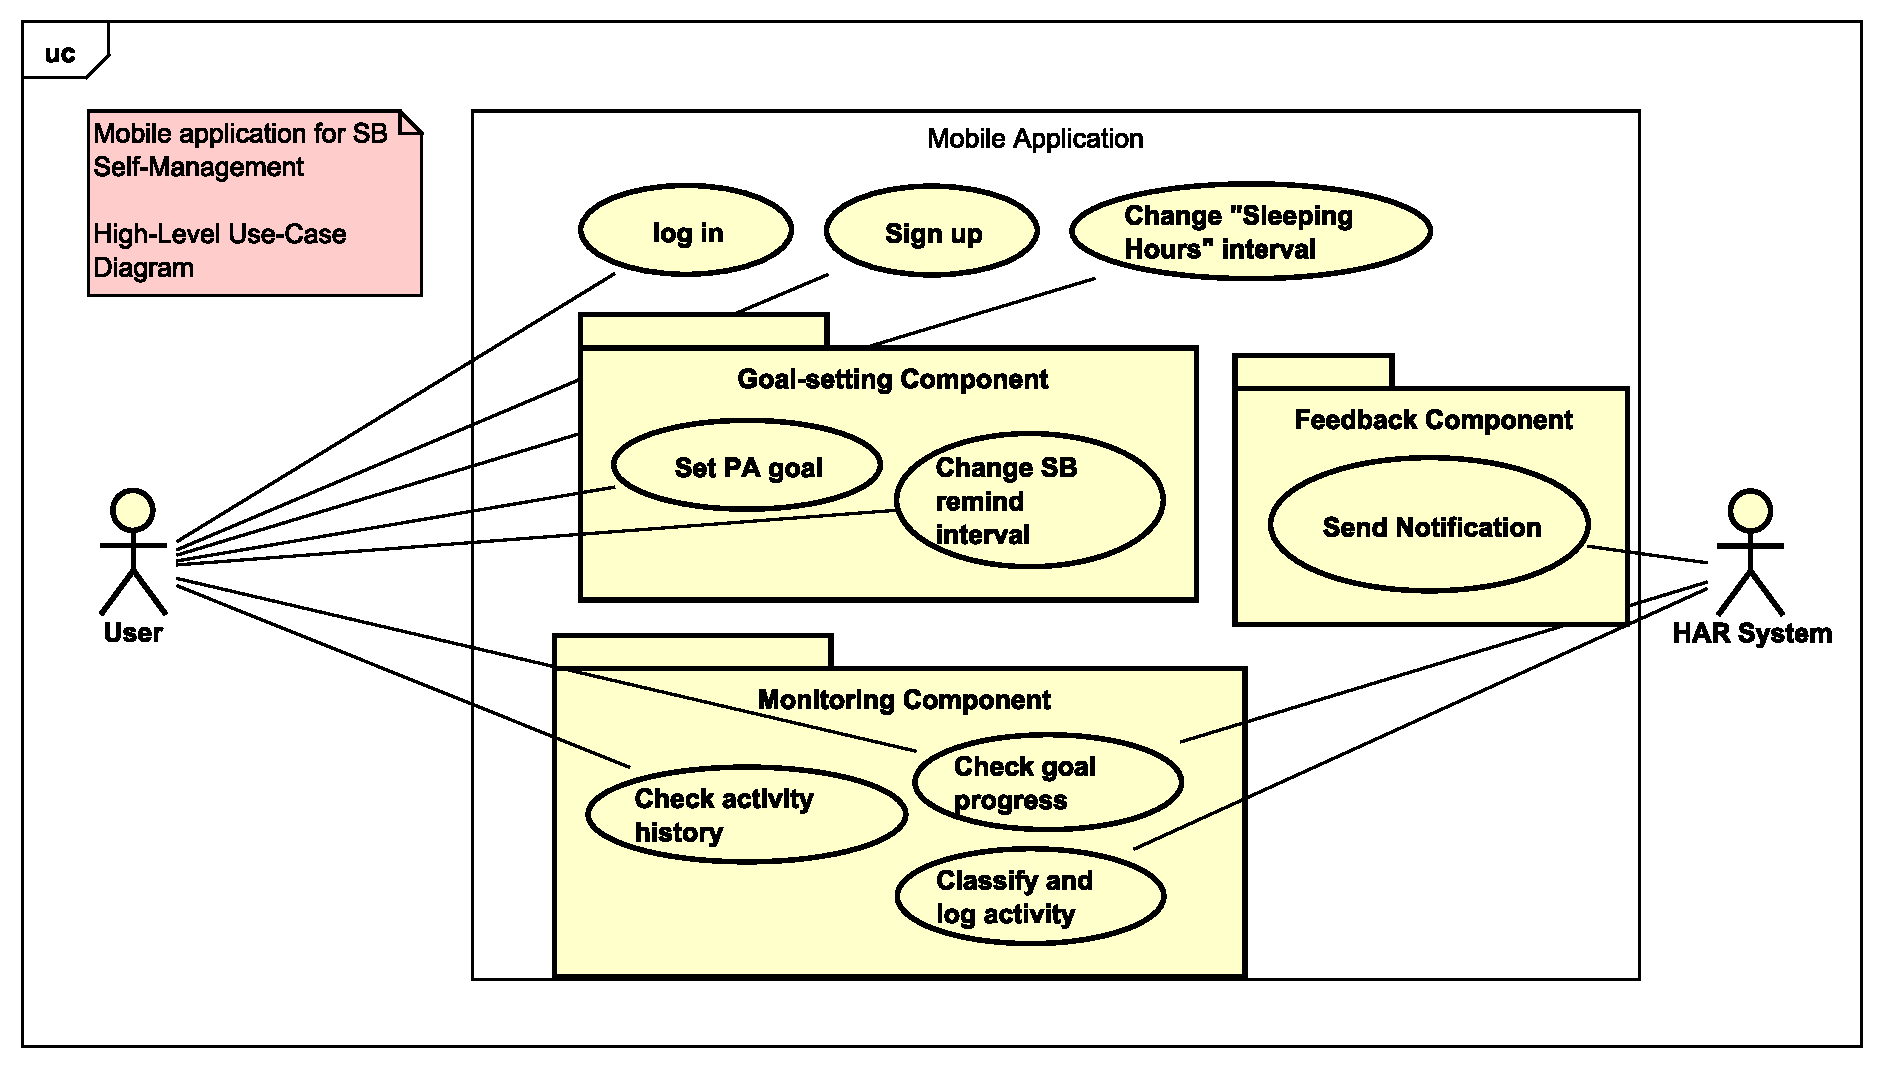
\includegraphics[width=15cm]{use_case_diagram}
        \caption{Use case diagram of \textit{"Active Minutes"}}
        \label{fig:use-case-diagram}
    \end{figure}
    
    \subsection{Goal-Setting Component}
    \label{section-goal-setting-component}
    Goal-setting is an important aspect of the self-management and behaviour change process. This component's requirements have been informed by the British Heart Foundation \citep[14]{townsend2015}, e.g.\ a minimum of 30 minutes of \gls{pa} is used as a guideline. The software implementation allows the user to set goals which become a target in the first step towards behaviour change and better lifestyle.
    
    \begin{enumerate}
        \item \gls{gsc} shall allow the user to set a \gls{pa} goal
        \begin{enumerate}
            \item \gls{gsc} shall provide list of recommended \gls{pa} goals
            \item \gls{gsc} shall automatically set the recommended \gls{pa} goal if the user does not explicitly do so 
        \end{enumerate}
        \item \gls{gsc} shall allow the user to set a Sedentary Time (\gls{st}) goal
        \begin{enumerate}
            \item \gls{gsc} shall allow the user to set a Maximum Continuous Inactivity (MCI) before a reminding notification is sent 
        \end{enumerate}
    \end{enumerate}
    
    
    \subsection{Monitoring component}
    \label{subsection:monitoring-component}
    The main purpose of the \gls{mc} is to continuously recognise activities and analyse the levels of \gls{pa} and \gls{st}. The following requirements have been derived from analysing past and current mobile devices as well as from discussions with the client.
    
    \begin{enumerate}
        \item The \gls{mc} component shall classify physical activities
        \begin{enumerate}
            \item HAR component shall recognise the following activities:
            \begin{enumerate}
                \item walking;
                \item running;
                \item cycling;
                \item static
            \end{enumerate}
        \end{enumerate}
        \item The \gls{mc} component shall analyse and aggregate user's \gls{pa} and \gls{st} amounts in real time
            \begin{enumerate}
                \item \gls{mc} shall increment user's \gls{pa} or \gls{st} value whenever physical activity or sedentary behaviour is recognised
            \end{enumerate}
        \item The \gls{mc} shall personalise \gls{har}'s classifier
            \begin{enumerate}
                \item When enough user data is collected, the system shall retrain the classifier combining the general data collected from the project participants with user's own data. According to \citet[376]{arapakis_athanasakos_jose_2010}, that is expected to improve the classifier's classification accuracy.
            \end{enumerate}
            
        \item \gls{mc} shall keep history of previously accumulated \gls{pa} and \gls{st} amounts
            \begin{enumerate}
                \item The system shall allow the user to group the collected data in "Daily" and "Weekly" representation
            \end{enumerate}
        
        \item The user shall be able to set the \textit{Sleeping Hours Time Interval} (\gls{shti}) during which no measurement of \gls{pa} or \gls{st} should occur
      
    \end{enumerate}
    
    \subsection{Feedback Component}
    \label{section:feedback-component}
    The \gls{fc} is responsible for sending notifications to the user. It can provide important information such as when a previously set goal is attained or reminder for the user that they are spending too much static time.
    \begin{enumerate}
        \item \gls{fc} shall notify the user when they are being sedentary for 1 hour (or the value set by the user) as recommended by \citet[]{swartz2011}
        
        \item \gls{fc} shall notify the user when a previously set goal is attained (e.g. being active for 30 minutes)
        
        \item \gls{fc} shall not send notifications during the user set "Sleeping Hours" time interval (e.g. 20:00 - 8:00).
        
        \item \gls{fc} shall send a notification to the user every Sunday to show goal-performance feedback for the past week
           
    \end{enumerate}

\section{Non-functional Requirements}
The mobile application proposed in this work has to comply with a number of additional requirements. According to \citet[87]{sommerville2010}, Non-functional are those requirements that do not concern the system directly. They apply to the whole system such as performance and security.  Since the \gls{gsc}, \gls{mc} and \gls{fc} are all part of the same software, their non-functional requirements will be discussed all together.
    
    \subsection{Accuracy}
    The accuracy of the system is measured as the \textit{Active}/\textit{Static} error rate rather than  the classification accuracy of the classifier on specific activity classes e.g. cycling. The system shall minimise errors where an activity of type \textit{Active} is misclassified as type \textit{Static} and vice versa since that would lead to incorrect PA daily readings and user may be doing less physical activity if they are notified incorrectly for attained goal.  The Active/Static error rate shall be less than 10\%. This number has been chosen based on two reasons. First, that error rate can only have a small effect on goal achievement,  for example, if we consider a user with a goal of 30 minutes PA and a 10\% error that gives us 27 minutes of PA (30 - 30*0.1) which is still close to the initial 30 minutes goal. Second, this error rate amount is achievable within the time constraints of the project.
    
    \subsection{Battery consumption}
    Since the resources of every portable device (i.e. mobile phone) are constrained, the system shall be designed so that it consumes a reasonable amount of battery power. The device shall be able to function without the need for a charge for at least 12 hours. For example, the user must not need to charge the device in the middle of the day as this would prevent the \gls{mc} from monitoring activity.
    
    \subsection{Security}
    The mobile application shall store user data only on the system in order to minimise the risk of data breach. In addition, the following considerations have been taken into account:
    
    \begin{enumerate}
        \item The system shall show authentication screen before showing any data such as how active the user has been during the day
        \item The system shall encrypt the data stored in a local database
    \end{enumerate}
    
    \subsection{System Quality Attributes}
    \label{section:system-quality-attributes}
        \subsubsection{Adaptability}
        Modern mobile applications should be able to quickly adapt to new requirements as the market changes. The intention is to achieve adaptability by implementing the \gls{mvp} software development pattern. That allows the system to incorporate new features easily as the system is separated into loosely coupled logical parts.
        
        \subsubsection{Scalability}
        The system should be scalable to accommodate large amounts of data collected by different users. For example, the system should be able to handle the data for at least five users.
        
        \subsubsection{Modularity}
        As living in a fast-changing world, user requirements can change quickly in a short period of time. Thus, the system should be able to change or replace features so it can adapt to change. For example, each mobile screen's logic is encapsulated in a separate directory which can be interchanged easily without affecting the integrity of the system.  
        
        \subsubsection{Testability}
        Testing any system is crucial since it allows the discovery of unwanted system behaviours. To assure that the system works as intended, the system shall be tested by both assertions and Quality Assurance tests. 
        
        \subsubsection{Maintainability}
        As with every software product, the need for maintains is unavoidable. Thus, to ease this process, the system shall be designed in such a way so that it allows for easy evolution. For example, extending the system by adding new features.
        
        \subsubsection{Robustness}
        Since the system requires a constant monitoring of the user (e.g. collecting contextual data), it is imperative that the system encompasses as many points of failure as possible. Thus the system shall be taken through series of QA tests as well as unit tests to minimise the points of failure. 
    
    
    